\section{Effekt Hacks}

Dieser Abschnitt soll sich der Umsetzung unterschiedlicher Animationen, Formen und Effekte der Seite in CSS widmen. Dabei sollen diese nicht auf den Einsatz von Javascript angewiesen sein, werden aber durch dessen Einsatz aufgewertet.
Es werden vor allem CSS3 Transitions für Animationen und die Pseudoelemente :before und :after für Formen eingesetzt.
\subsection{Menübutton}
\subsubsection{Grundüberlegung}

\begin{figure} [h]
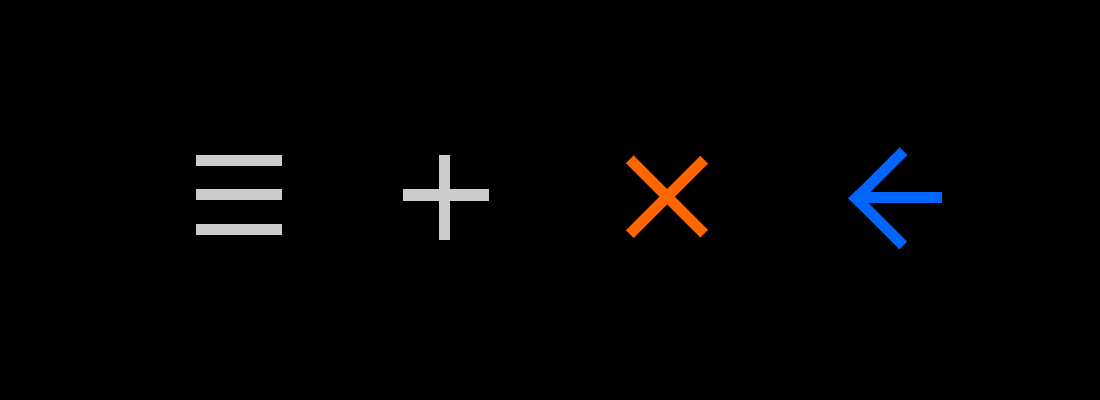
\includegraphics[width=\textwidth]{./img/css_buttons1.png}
\caption{Die 4 Zustände des CSS Menübuttons}
\label{css_buttons1}
\end{figure}

Das Animationstechnische Highlight der Seite ist der Menübutton oben links neben dem Digital Home Logo. Er zeigt im Normalzustand drei Striche, die auf einigen Websites als Menüsymbol eingesetzt werden. Hovert man den Menübutton, so transformieren sich der erste und der zweite Strich zu einem Plus, während der dritte Strich ausgeblendet wird. Wichtig ist dabei der weiche Übergang, damit der User das Plus nicht als neues Element wahrnimmt, sondern als Feedback auf seine Interaktion mit dem Menübutton. Nur auf diesem Weg kann er den Menübutton auch als Schaltfläche wahrnehmen und richtig mit dieser interagieren. Abgesehen von der Hover-transformation muss der User auch ein Feedback bekommen, wenn er auf den Button klickt. Dabei ändert sich der Zustand des Buttons.

Nun sieht man im Normalzustand ein orangenes Kreuz, während im Hoverzustand ein blauer Pfeil zu sehen ist. Diese Formen (in Abbildung \ref{css_buttons1} zu sehen) sind bewusst gewählt worden. Die drei Striche suggerieren eine Liste, die abgerufen werden kann. In diesem Fall ist das Menü die Liste. Das Plus deutet auf einen Zuwachs hin. Fährt das Menü von links in das Bild, so wächst zum einen seine sichtbare Größe (von 0 zu seiner eigentlichen). Dazu wurde der Bildschirm um ein Element bereichert, also ist die Anzahl der Elemente „gewachsen“. Zuletzt zeigt das Menü im ausgefahrenen Zustand die Überschriften der Symbole in der Menüleiste (Desktop) bzw. zeigt dem Nutzer Navigationsmöglichkeiten (Mobile). Für den User stellt dies einen Informationszuwachs dar.

Das Kreuz bedeutet „Beenden“. Es wird z.B. in Betriebssystemen als Symbol zum Schließen einer Anwendung verwendet oder um einen Vorgang abzubrechen. Hier soll der Nutzer sehen, dass er das Menü über die Schaltfläche wieder schließen kann. Da man damit jedoch ein Element aus dem Bild entfernt, wurde das Kreuz orange gefärbt, um den Nutzer vor jener Handlung zu warnen und den Button auffälliger zu machen. Der User soll damit nicht davon abgehalten werden, das Menü wieder zu schließen, vielmehr soll die Warnung als Vorwarnung verstanden werden. Dadurch erwartet der Nutzer das Verschwinden des Menüs und wird nicht überrascht.

An dieser Stelle sollte erwähnt werden, warum zwei Aktionen auf einen Button gelegt wurden. Man hätte alternativ auch im Menü einen separaten „Schließen“-Button integrieren können. Der User hätte dann auf den Menübutton geklickt, das Menü hätte sich geöffnet. Dann hätte er den „Schließen“-Button aber erst suchen müssen, um dann zu überlegen, wo der Unterschied zwischen den beiden Schaltflächen liegt. Zusätzlich hätte er seine Maus bewegen müssen, was dem Nutzer Raum gibt, um sich zu verklicken und unbeabsichtigt auf eine andere Seite zu kommen. Dadurch würde sich der Nutzer ziemlich ärgern, da solche Situationen hätten vermieden werden können. Zuletzt kommt erschwerend dazu, dass man von Kindesbeinen daran gewöhnt wird, zwei komplementäre Aktionen über einen Knopf auszuführen. PCs (auch alle anderen elektronischen Geräte) besitzen beispielsweise einen einzelnen Knopf, über den man das Gerät ein- und ausschaltet, gleichermaßen haben Kugelschreiber einen Knopf, mit dem man die Miene ein- und ausfahren kann. Wir benutzen die Türklinke, um die Tür zu öffnen, wir benutzen die gleiche Türklinke, um die Tür wieder zu schließen. Wir können also davon ausgehen, das  eine kontextsensitive (dynamische) Schaltfläche dem Nutzer sehr viel vertrauter ist als zwei statische (`Öffnen` und `Schließen`).

Der blaue Pfeil soll dem Nutzer verdeutlichen, dass eine Bewegung passieren wird, nämlich nach links. Damit wird die Bedeutung des Kreuzes nochmals unterstrichen, der Pfeil weist den Nutzer explizit darauf hin, dass beim Anklicken das Element, mit dem interagiert wird (das Menü), nach links verschwinden wird. Da links die Richtung ist, wo die Menüleiste herkommt, wird der Pfeil nach links mit der Wiederherstellung eines Anfangszustandes assoziiert.


\subsubsection{Code}

\begin{figure} [h]
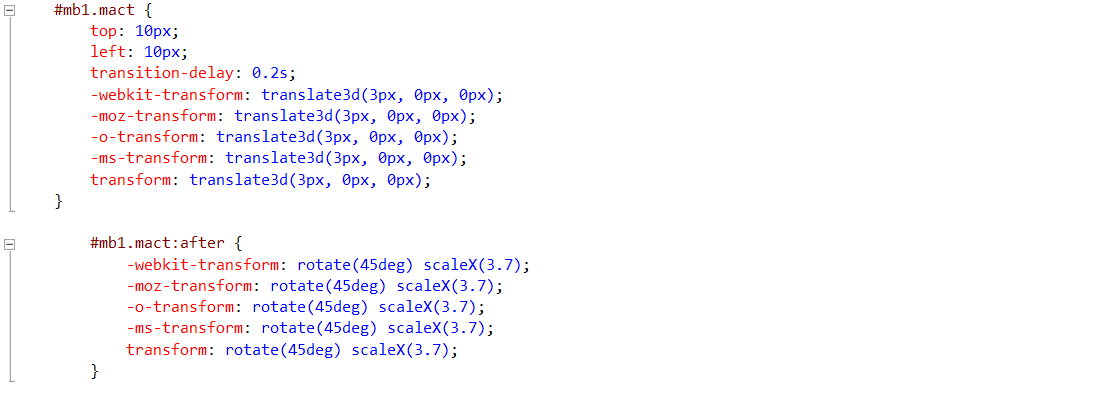
\includegraphics[width=\textwidth]{./img/css_after.png}
\caption{Die Trennung von rotate() und translate()}
\label{css_after}
\end{figure}
Die Linien des Menübuttons sind <div> Container. Zur Drehung der Objekte werden CSS3 Transforms verwendet. Speziell die Funktionen rotate() und translate3d(). Die Kombination der beiden in einem Element ist jedoch Problematisch, da sich mit rotate() die Objektmatrix verändert und mit translate() die Objektachse nicht verschoben wird. Ein gedrehtes Objekt können wir also nicht entlang der ursprünglichen X-/Y-Achsen verschieben und ein verschobenes Objekt dreht sich immernoch um seine ursprüngliche Achse. Hier kommt das Pseudoelement :after ins Spiel. Der Container arbeitet als Träger für das :after Element, welches durch seine absolute Positionierung einen eigenen Container bildet (Dies gilt jedoch nicht für den Suchbutton, da er weitaus weniger komplex ist und jenes Verhalten zudem für die Animation nützlich ist), wie in Abbildung \ref{css_after} zu sehen. Der Träger wird durch Translation verschoben, das darin enthaltene :after Element dreht sich dann um die scheinbar verschobene Objektachse.


Durch Versuche wurden 0.4 Sekunden als optimale Zeit ausgemacht. Um die Animation organischer wirken zu lassen, wird „ease“ als CSS Easingfunktion verwendet. Dazu kommen variierende transition-delays, die die Animation etwas auflockern.
Zur Translation im zweidimensionalen Raum reicht translate() eigentlich aus, mit translate3d() soll jedoch eine Hardwarebeschleunigung forciert werden (Quelle: \url{http://davidwalsh.name/translate3d}).

\subsection{link:before}

\subsection{Metro Kacheln}
[CSS3 Columns]
\subsection{schräge Kanten}
\begin{figure} [h]
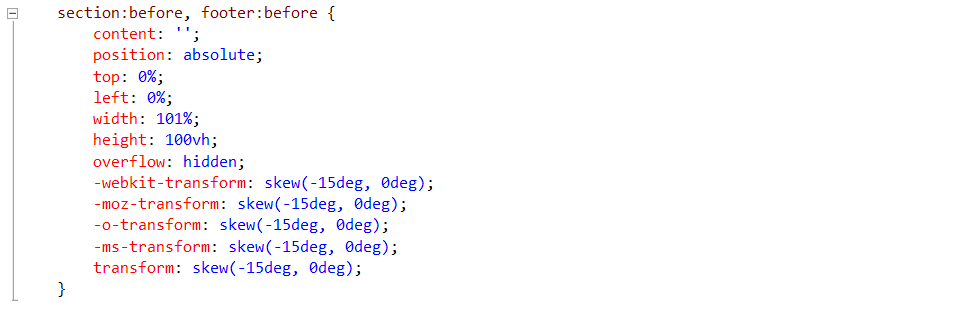
\includegraphics[width=\textwidth]{./img/css_secbefore.png}
\caption{Der Hintergrund der Section als Container}
\label{css_secbefore}
\end{figure}
Für die schrägen Kanten der Sections wurden die :before Elemente und absolute Positionierung genutzt (siehe Abbildung \ref{css_secbefore}). Damit kann die Neigung und das Aussehen des Hintergrundes von der des Vordergrundes getrennt werden, sodass der Hintergrund ohne Auswirkungen auf das Floaten des Contents oder der Sections gestaltet werden kann. Um Kantenglättungsrelikten aus dem Weg zu gehen, wurde die Breite des Hintergrunds auf 101\% gesetzt.
